\expandafter\let\csname ver@amssymb.sty\endcsname\empty
\documentclass[serif]{beamer}
\expandafter\let\csname ver@amssymb.sty\endcsname\relax
\usepackage{etex}
\usepackage[bitstream-charter]{mathdesign} % Use BT Charter font
\usepackage[T1]{fontenc}                   % Use T1 encoding instead of OT1
\usepackage[utf8]{inputenc}                % Use UTF8 input encoding
\usepackage{microtype}                     % Improve typography
\usepackage{booktabs}
\usepackage{cancel}
\usepackage{algorithm}
\usepackage{algorithmicx}
\usepackage{algpseudocode}
\usepackage{hyperref}
\hypersetup{pdfstartview=Fit}
\usepackage{tikz}
\usetikzlibrary{shapes,snakes,shadows,arrows,calc}
\usetikzlibrary{decorations.markings}
\usepackage{multirow}
\usepackage{animate}
\usepackage{moresize}
\usepackage{colortbl}
\usepackage{xcolor}
\usepackage{amsmath}
\usepackage{etoolbox}
\usepackage{listings}
\usepackage{alltt}
\usepackage{textpos}

\renewcommand\footnotemark{}

\lstset{
  basewidth=0.5em,
%  columns=fullflexible,
  showspaces=false,
  showtabs=false,
  showstringspaces=false,
  commentstyle=\color{gray}\upshape,
}
\lstset{language=bash,frame=single,basicstyle=\ttfamily\footnotesize}
\lstdefinelanguage{XML}
{
  backgroundcolor=\color{gray!20},
  basicstyle=\ttfamily\ssmall,
  morestring=[b]",
  frame=single,
% morestring=[s]{>}{<},
  morecomment=[s]{<?}{?>},
  morecomment=[s]{<!--}{-->},
  stringstyle=\color{red},
  identifierstyle=\color{darkblue},
  keywordstyle=\color{cyan},
}

\definecolor{gray}{rgb}{0.4,0.4,0.4}
\definecolor{darkblue}{rgb}{0.0,0.0,0.6}
\definecolor{cyan}{rgb}{0.0,0.6,0.6}

\newcommand{\tikzmark}[1]{\tikz[overlay,remember picture] \node (#1) {};}
\newcommand*{\DrawArrow}[3][]{%
    % #1 = draw options
    % #2 = left point
    % #3 = right point
    \begin{tikzpicture}[overlay,remember picture]
        \draw [-latex, #1] ($(#2)+(0.3em,-1ex)$) to ($(#3)+(0,0.5ex)$);
    \end{tikzpicture}%
}

\usetheme{Copenhagen}
\usecolortheme{beaver}

\title{OpenMC Module: Detailed Geometry Specification and Visualization}
\author{\emph{Computational Reactor Physics Group}}
\date{\normalsize Department of Nuclear Science and Engineering\\
                  Massachusetts Institute of Technology \\
~\\
\tiny{This work is licensed under the Creative Commons Attribution-ShareAlike 3.0 Unported License. To view a copy of this license, visit http://creativecommons.org/licenses/by-sa/3.0/.}}

% Set Logo
\logo{
\includegraphics[scale=0.2]{src/crpg.png}\hspace*{8cm}

\includegraphics[scale=0.2,trim=0cm 3.0cm 2.2cm 0cm, clip=true]{src/mitlogo.pdf}}

\usenavigationsymbolstemplate{}

%-------------------------------------------------------------------------------
\begin{document}
%-------------------------------------------------------------------------------

\frame{\titlepage}\logo{} % remove logo after title page


%-------------------------------------------------------------------------------

\begin{frame}{Building Complex Models is Straightforward}
  \begin{columns}
    \begin{column}{0.5\linewidth}
      \begin{itemize}
        \item Universes
        \item Lattices
        \item Building a full-core model
        \item Visualizing geometry
      \end{itemize}
    \end{column}
    \begin{column}{0.5\linewidth}
      \centering
      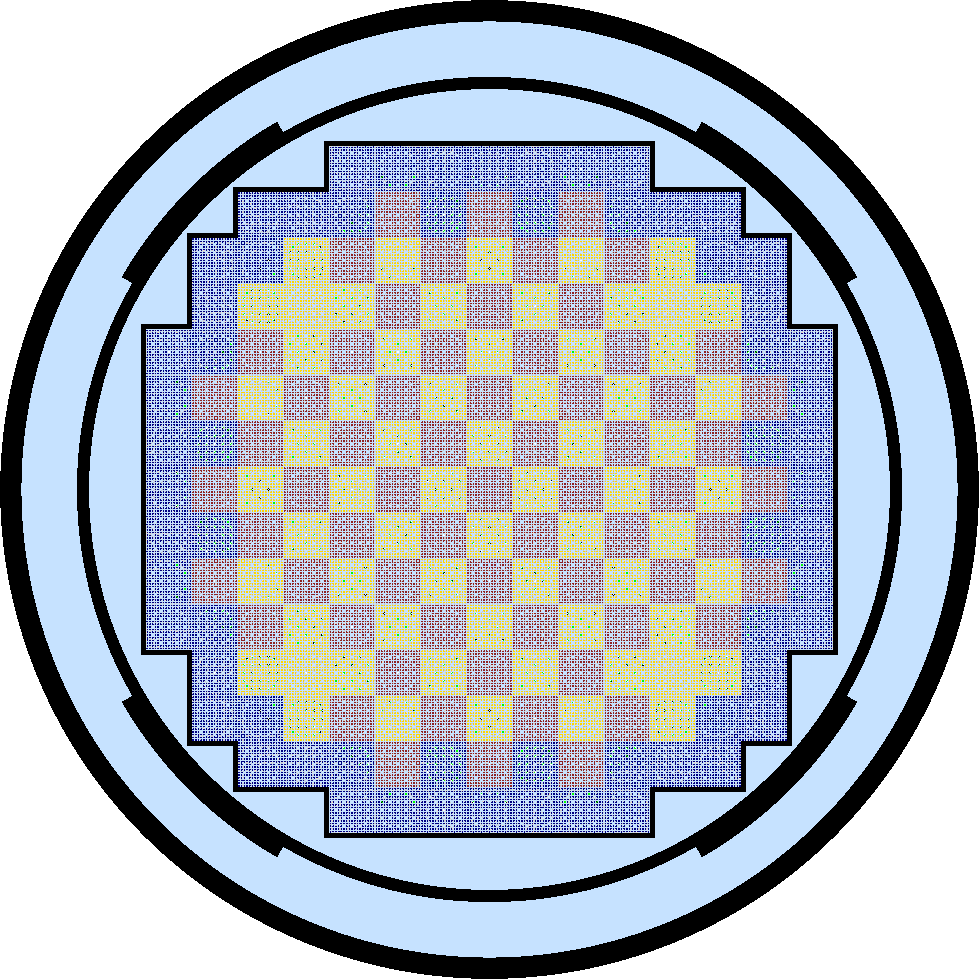
\includegraphics[width=2in]{src/core.png}      
    \end{column}
  \end{columns}
\end{frame}

%-------------------------------------------------------------------------------

\begin{frame}[fragile]{It's Easy to Hierarchically Build Models with Universes}

  \begin{scriptsize}
    \begin{lstlisting}[language=XML,gobble=4]
      <?xml version="1.0" encoding="UTF-8"?>
      <geometry>

        <!-- Fuel Rod Pincell Universe -->
        <surface id="1"  type="z-cylinder" coeffs="0.0 0.0 0.39218"/>     <!-- fuel OR   -->
        <surface id="2"  type="z-cylinder" coeffs="0.0 0.0 0.40005"/>     <!-- gap OR    -->
        <surface id="3"  type="z-cylinder" coeffs="0.0 0.0 0.45720"/>     <!-- clad OR   -->
        <cell id="21" universe="2" material="2" surfaces="  -1"/>         <!-- fuel  -->
        <cell id="22" universe="2" material="3" surfaces="1 -2"/>         <!-- clad  -->
        <cell id="23" universe="2" material="1" surfaces="   2"/>         <!-- water -->

      </geometry>
    \end{lstlisting}
  \end{scriptsize}


  \begin{itemize}
    \item Instead of using a \textit{material}, cells can be \textit{filled} with a universe
    \item By default universes share the same global coordinate system
    \begin{itemize}
      \item Can be translated and rotated - e.g. in lattices
    \end{itemize}
    \item Universes \textbf{must} be defined for \textbf{all} space
    \begin{itemize}
      \item Or you may encounter particle tracking errors!
    \end{itemize}
    \item Provides the easiest way to define multiple pincells, lattices, and 
    more complicated structures
  \end{itemize}


\end{frame}

%-------------------------------------------------------------------------------

\begin{frame}[fragile]{Cell Filling Example}


  \begin{scriptsize}
    \begin{lstlisting}[language=XML,gobble=4]
      <?xml version="1.0" encoding="UTF-8"?>
      <geometry>

        <!-- Fuel Rod Pincell Universe -->
        <surface id="1"  type="z-cylinder" coeffs="0.0 0.0 0.39218"/>     <!-- fuel OR   -->
        <surface id="2"  type="z-cylinder" coeffs="0.0 0.0 0.40005"/>     <!-- gap OR    -->
        <surface id="3"  type="z-cylinder" coeffs="0.0 0.0 0.45720"/>     <!-- clad OR   -->
        <cell id="21" universe="2" material="2" surfaces="  -1"/>         <!-- fuel  -->
        <cell id="22" universe="2" material="3" surfaces="1 -2"/>         <!-- clad  -->
        <cell id="23" universe="2" material="1" surfaces="   2"/>         <!-- water -->

        <!-- Main Universe -->
        <surface id="4"  type="x-plane" coeffs="-0.62992" boundary="reflective"/>
        <surface id="5"  type="x-plane" coeffs=" 0.62992" boundary="reflective"/>
        <surface id="6"  type="y-plane" coeffs="-0.62992" boundary="reflective"/>
        <surface id="7"  type="y-plane" coeffs=" 0.62992" boundary="reflective"/>
        <surface id="8"  type="z-plane" coeffs="-5.00000" boundary="reflective"/>
        <surface id="9"  type="z-plane" coeffs=" 5.00000" boundary="reflective"/>
        <cell id="1" universe="0" fill="2" surfaces="4 -5 6 -7 8 -9" />


      </geometry>
    \end{lstlisting}
  \end{scriptsize}

  \centering
  \begin{tikzpicture}
    \fill[white] (-1,-1) rectangle (9,1);
    \draw[fill=blue!50!white] (-1,-1) rectangle (1,1);
    \node at (0,0) {\small Cell 1};
    \draw[->,thick] (1.2,0) -- (3.8,0);
    \draw[fill=blue!70!white] (4,-1) rectangle (6,1);
    \draw[fill=gray] (5,0) circle (0.7258);
    \draw[fill=yellow] (5,0) circle (0.63508);
    \draw[fill=red] (5,0) circle (0.62250);
    \node[align=center] at (7.5,0) {\small Filled by \\ \small Universe 2};
  \end{tikzpicture}

\end{frame}

%-------------------------------------------------------------------------------

\begin{frame}[fragile]{Cell Filling Example}


  \begin{scriptsize}
    \begin{lstlisting}[language=XML,gobble=4]
      <?xml version="1.0" encoding="UTF-8"?>
      <geometry>

        <!-- Fuel Rod Pincell Universe -->
        <surface id="1"  type="z-cylinder" coeffs="0.0 0.0 0.39218"/>     <!-- fuel OR   -->
        <surface id="2"  type="z-cylinder" coeffs="0.0 0.0 0.40005"/>     <!-- gap OR    -->
        <surface id="3"  type="z-cylinder" coeffs="0.0 0.0 0.45720"/>     <!-- clad OR   -->
        <cell id="21" universe="2" material="2" surfaces="  -1"/>         <!-- fuel  -->
        <cell id="22" universe="2" material="3" surfaces="1 -2"/>         <!-- clad  -->
        <cell id="23" universe="2" material="1" surfaces="   2"/>         <!-- water -->

        <!-- Main Universe -->
        <surface id="4"  type="x-plane" coeffs="-0.0"     boundary="reflective"/>
        <surface id="5"  type="x-plane" coeffs=" 0.62992" boundary="reflective"/>
        <surface id="6"  type="y-plane" coeffs="-0.62992" boundary="reflective"/>
        <surface id="7"  type="y-plane" coeffs=" 0.62992" boundary="reflective"/>
        <surface id="8"  type="z-plane" coeffs="-5.00000" boundary="reflective"/>
        <surface id="9"  type="z-plane" coeffs=" 5.00000" boundary="reflective"/>
        <cell id="1" universe="0" fill="2" surfaces="4 -5 6 -7 8 -9" />


      </geometry>
    \end{lstlisting}
  \end{scriptsize}

  \centering
  \begin{tikzpicture}
    \fill[white] (-1,-1) rectangle (9,1);
    \draw[fill=white, dashed] (-1,-1) rectangle (0,1);
    \draw[fill=blue!50!white] (0,-1) rectangle (1,1);
    \node[rotate=90] at (0.5,0) {\small Cell 1};
    \draw[->,thick] (1.2,0) -- (3.8,0);
    \draw[fill=white, dashed] (4,-1) rectangle (5,1);
    \begin{scope}
      \clip (5,-1) rectangle (6,1);
      \draw[fill=blue!70!white] (4,-1) rectangle (6,1);
      \draw[fill=gray] (5,0) circle (0.7258);
      \draw[fill=yellow] (5,0) circle (0.63508);
      \draw[fill=red] (5,0) circle (0.62250);
    \end{scope}
    \node[align=center] at (7.5,0) {\small Smaller cells \\ \small clip universes};
  \end{tikzpicture}

\end{frame}


%-------------------------------------------------------------------------------

\begin{frame}[fragile]{Cell Filling Example}

  \begin{scriptsize}
    \begin{lstlisting}[language=XML,gobble=4]
      <?xml version="1.0" encoding="UTF-8"?>
      <geometry>

        <!-- Fuel Rod Pincell Universe -->
        <surface id="1"  type="z-cylinder" coeffs="0.0 0.0 0.39218"/>     <!-- fuel OR   -->
        <surface id="2"  type="z-cylinder" coeffs="0.0 0.0 0.40005"/>     <!-- gap OR    -->
        <surface id="3"  type="z-cylinder" coeffs="0.0 0.0 0.45720"/>     <!-- clad OR   -->
        <cell id="21" universe="2" material="2" surfaces="  -1"/>         <!-- fuel  -->
        <cell id="22" universe="2" material="3" surfaces="1 -2"/>         <!-- clad  -->
        <cell id="23" universe="2" material="1" surfaces="   2"/>         <!-- water -->

        <!-- Main Universe -->
        <surface id="4"  type="x-plane" coeffs="-0.0"     boundary="reflective"/>
        <surface id="5"  type="x-plane" coeffs=" 0.62992" boundary="reflective"/>
        <surface id="6"  type="y-plane" coeffs="-0.62992" boundary="reflective"/>
        <surface id="7"  type="y-plane" coeffs=" 0.62992" boundary="reflective"/>
        <surface id="8"  type="z-plane" coeffs="-5.00000" boundary="reflective"/>
        <surface id="9"  type="z-plane" coeffs=" 5.00000" boundary="reflective"/>
        <cell id="1" universe="0" fill="2" surfaces="4 -5 6 -7 8 -9"
                                           translation="0.31496 0.0 0.0" />

      </geometry>
    \end{lstlisting}
  \end{scriptsize}

  \centering
  \begin{tikzpicture}
    \fill[white] (-1,-1) rectangle (9,1);
    \draw[fill=white, dashed] (-1,-1) rectangle (0,1);
    \draw[fill=blue!50!white] (0,-1) rectangle (1,1);
    \node[rotate=90] at (0.5,0) {\small Cell 1};
    \draw[->,thick] (1.2,0) -- (3.8,0);
    \draw[fill=white, dashed] (4,-1) rectangle (5,1);
    \begin{scope}
      \clip (5,-1) rectangle (6,1);
      \begin{scope}[shift={(0.5,0)}]
        \draw[fill=blue!70!white] (4,-1) rectangle (6,1);
        \draw[fill=gray] (5,0) circle (0.7258);
        \draw[fill=yellow] (5,0) circle (0.63508);
        \draw[fill=red] (5,0) circle (0.62250);
      \end{scope}
    \end{scope}
    \node[align=center] at (7.5,0) {\small Fills can \\ \small be translated};
  \end{tikzpicture}

\end{frame}

%-------------------------------------------------------------------------------

\begin{frame}[fragile]{Cell Filling Example}


  \begin{scriptsize}
    \begin{lstlisting}[language=XML,gobble=4]
      <?xml version="1.0" encoding="UTF-8"?>
      <geometry>

        <!-- Fuel Rod Pincell Universe -->
        <surface id="1"  type="z-cylinder" coeffs="0.0 0.0 0.39218"/>     <!-- fuel OR   -->
        <surface id="2"  type="z-cylinder" coeffs="0.0 0.0 0.40005"/>     <!-- gap OR    -->
        <surface id="3"  type="z-cylinder" coeffs="0.0 0.0 0.45720"/>     <!-- clad OR   -->
        <cell id="21" universe="2" material="2" surfaces="  -1"/>         <!-- fuel  -->
        <cell id="22" universe="2" material="3" surfaces="1 -2"/>         <!-- clad  -->
        <cell id="23" universe="2" material="1" surfaces="   2"/>         <!-- water -->

        <!-- Main Universe -->
        <surface id="4"  type="x-plane" coeffs="-0.0"     boundary="reflective"/>
        <surface id="5"  type="x-plane" coeffs=" 0.62992" boundary="reflective"/>
        <surface id="6"  type="y-plane" coeffs="-0.62992" boundary="reflective"/>
        <surface id="7"  type="y-plane" coeffs=" 0.62992" boundary="reflective"/>
        <surface id="8"  type="z-plane" coeffs="-5.00000" boundary="reflective"/>
        <surface id="9"  type="z-plane" coeffs=" 5.00000" boundary="reflective"/>
        <cell id="1" universe="0" fill="2" surfaces="4 -5 6 -7 8 -9"
                                           translation="0.31496 0.0 0.0"
                                           rotation="90.0 0.0 0.0" />
      </geometry>
    \end{lstlisting}
  \end{scriptsize}

  \centering
  \begin{tikzpicture}
    \fill[white] (-1,-1) rectangle (9,1);
    \draw[fill=white, dashed] (-1,-1) rectangle (0,1);
    \draw[fill=blue!50!white] (0,-1) rectangle (1,1);
    \node[rotate=90] at (0.5,0) {\small Cell 1};
    \draw[->,thick] (1.2,0) -- (3.8,0);
    \draw[fill=white, dashed] (4,-1) rectangle (5,1);
    \begin{scope}
      \clip (5,-1) rectangle (6,1);
      \begin{scope}[shift={(0.5,0)}]
        \draw[fill=blue!70!white] (4,-1) rectangle (6,1);
        \draw[fill=gray] (5,0) circle (0.7258);
        \draw[fill=yellow] (5,0) circle (0.63508);
        \draw[fill=red] (5,0) circle (0.62250);
        \draw[->,thick] (5,0.3) arc[radius=0.3, start angle=90, end angle=0];
      \end{scope}
    \end{scope}m
    \node[align=center] (la) at (7.5,0) {\small Fills can \\ \small be rotated};
    \node[align=center,anchor=north] at (la.south) {\tiny Rotation is always first!};
  \end{tikzpicture}

\end{frame}


%-------------------------------------------------------------------------------

\begin{frame}[fragile]{Lattices Automate Filling of Repetitive Structures}

  \begin{scriptsize}
    \begin{lstlisting}[language=XML,gobble=4]
      <?xml version="1.0" encoding="UTF-8"?>
      <geometry>

        <!-- Fuel Rod Pincell Universe -->
        <surface id="1"  type="z-cylinder" coeffs="0.0 0.0 0.39218"/>     <!-- fuel OR   -->
        <surface id="2"  type="z-cylinder" coeffs="0.0 0.0 0.40005"/>     <!-- gap OR    -->
        <surface id="3"  type="z-cylinder" coeffs="0.0 0.0 0.45720"/>     <!-- clad OR   -->
        <cell id="21" universe="2" material="2" surfaces="  -1"/>         <!-- fuel  -->
        <cell id="22" universe="2" material="3" surfaces="1 -2"/>         <!-- clad  -->
        <cell id="23" universe="2" material="1" surfaces="   2"/>         <!-- water -->

        <!-- Pin-Lattice -->
        <lattice id="100" type="rectangular" dimension="2 2">
          <lower_left> -1.25984 -1.25984 </lower_left>
          <width> 1.25984 1.25984 </width>
          <universes>
            2 2
            2 2
          </universes>
        </lattice>
        <surface id="99" type="sphere" coeffs="0.0 0.0 0.0 400.0"/>
        <cell id="1000" universe="0" fill="100" surfaces="-99"/>

      </geometry>
    \end{lstlisting}
  \end{scriptsize}


  \begin{itemize}
    \item \small Lattices set up a grid of cells filled by other universes, handling
    fill translation automatically
    \item \small Lattices are themselves very similar to universes - to use them, other
    cells must be filled with them
  \end{itemize}
  
  
  \onslide<2>{
    \setlength{\TPHorizModule}{\framewidth}
    \setlength{\TPVertModule}{\paperheight}
    \begin{textblock}{1}(0.67,-0.32)
      \begin{tikzpicture}
        \draw[red,thick,->](1,0) node (la) [,anchor=west] {Bad!} -- (.2,0);
        \node[red,anchor=north] at (la.south) {\footnotesize There is undefined space!};
      \end{tikzpicture}
    \end{textblock}
  }
  
\end{frame}

%-------------------------------------------------------------------------------

\begin{frame}[fragile]{Lattice Example}


  \begin{scriptsize}
    \begin{lstlisting}[language=XML,gobble=4]
      <?xml version="1.0" encoding="UTF-8"?>
      <geometry>

        <!-- Fuel Rod Pincell Universe -->
        <surface id="1"  type="z-cylinder" coeffs="0.0 0.0 0.39218"/>     <!-- fuel OR   -->
        <surface id="2"  type="z-cylinder" coeffs="0.0 0.0 0.40005"/>     <!-- gap OR    -->
        <surface id="3"  type="z-cylinder" coeffs="0.0 0.0 0.45720"/>     <!-- clad OR   -->
        <cell id="21" universe="2" material="2" surfaces="  -1"/>         <!-- fuel  -->
        <cell id="22" universe="2" material="3" surfaces="1 -2"/>         <!-- clad  -->
        <cell id="23" universe="2" material="1" surfaces="   2"/>         <!-- water -->

        <!-- Pin-Lattice -->
        <lattice id="100" type="rectangular" dimension="2 2">
          <lower_left> -1.25984 -1.25984 </lower_left>
          <width> 1.25984 1.25984 </width>
          <universes>
            2 2
            2 2
          </universes>
        </lattice>
        
        <!-- Main Universe -->
        <surface id="4"  type="x-plane" coeffs="-1.25984" boundary="reflective"/>
        <surface id="5"  type="x-plane" coeffs=" 1.25984" boundary="reflective"/>
        <surface id="6"  type="y-plane" coeffs="-1.25984" boundary="reflective"/>
        <surface id="7"  type="y-plane" coeffs=" 1.25984" boundary="reflective"/>
        <surface id="8"  type="z-plane" coeffs="-5.00000" boundary="reflective"/>
        <surface id="9"  type="z-plane" coeffs=" 5.00000" boundary="reflective"/>
        <cell id="1" universe="0" fill="100" surfaces="4 -5 6 -7 8 -9"/>
        
      </geometry>
    \end{lstlisting}
  \end{scriptsize}

  \onslide<1>{
    \setlength{\TPHorizModule}{\framewidth}
    \setlength{\TPVertModule}{\paperheight}
    \begin{textblock}{1}(0.86,-0.265)
      \begin{tikzpicture}
        \draw[green,thick,->](0.3,0) node[anchor=west] {Good!} -- (0,0);
        \draw[green] (-0.1,-.7) -- (0,-.7) -- (0,.8) -- (-0.1,.8);
      \end{tikzpicture}
    \end{textblock}
  }
  \onslide<2>{
    \setlength{\TPHorizModule}{\framewidth}
    \setlength{\TPVertModule}{\paperheight}
    \begin{textblock}{1}(0.635,-0.6)
      \begin{tikzpicture}
        \begin{scope}[shift={(-1,-1)}]
          \draw[fill=blue!70!white] (-1,-1) rectangle (1,1);
          \draw[fill=gray] (0,0) circle (0.7258);
          \draw[fill=yellow] (0,0) circle (0.63508);
          \draw[fill=red] (0,0) circle (0.62250);
        \end{scope}
        \begin{scope}[shift={(1,-1)}]
          \draw[fill=blue!70!white] (-1,-1) rectangle (1,1);
          \draw[fill=gray] (0,0) circle (0.7258);
          \draw[fill=yellow] (0,0) circle (0.63508);
          \draw[fill=red] (0,0) circle (0.62250);
        \end{scope}
        \begin{scope}[shift={(-1,1)}]
          \draw[fill=blue!70!white] (-1,-1) rectangle (1,1);
          \draw[fill=gray] (0,0) circle (0.7258);
          \draw[fill=yellow] (0,0) circle (0.63508);
          \draw[fill=red] (0,0) circle (0.62250);
        \end{scope}
        \begin{scope}[shift={(1,1)}]
          \draw[fill=blue!70!white] (-1,-1) rectangle (1,1);
          \draw[fill=gray] (0,0) circle (0.7258);
          \draw[fill=yellow] (0,0) circle (0.63508);
          \draw[fill=red] (0,0) circle (0.62250);
        \end{scope}
      \end{tikzpicture}
    \end{textblock}
  }
  

\end{frame}


%-------------------------------------------------------------------------------

\begin{frame}[fragile]{Now Let's Build a Core!}

  \begin{enumerate}
    \item<1-> Make all pincell universes
    \begin{itemize}
      \item<1-> Fuel rod, control rod, burnable absorber, etc.
    \end{itemize}
    \item<2-> Make assembly pin-lattices
    \begin{itemize}
      \item<2-> Different enrichment assemblies, different burnable absorber configurations, etc.
    \end{itemize}
    \item<3-> Make core assembly-lattice
  \end{enumerate}

  \centering
  \onslide<3->{See input xml files in examples/demos/plotting}
  
  \vspace{0.2cm}
  
  \centering
  \begin{tikzpicture}
    \onslide<1->\draw[fill=blue!70!white] (-1,-1) rectangle (1,1);
    \onslide<1->\draw[fill=gray] (0,0) circle (0.7258);
    \onslide<1->\draw[fill=yellow] (0,0) circle (0.63508);
    \onslide<1->\draw[fill=red] (0,0) circle (0.62250);

    \onslide<2->\draw[thick,->] (1.2,0) -- (2.0,0);
    \begin{scope}[shift={(5.3,0)}, transform canvas={scale=0.7}]
      \begin{scope}[shift={(-1,-1)}]
        \onslide<2->\draw[fill=blue!70!white] (-1,-1) rectangle (1,1);
        \onslide<2->\draw[fill=gray] (0,0) circle (0.7258);
        \onslide<2->\draw[fill=yellow] (0,0) circle (0.63508);
        \onslide<2->\draw[fill=green] (0,0) circle (0.62250);
      \end{scope}
      \begin{scope}[shift={(1,-1)}]
        \onslide<2->\draw[fill=blue!70!white] (-1,-1) rectangle (1,1);
        \onslide<2->\draw[fill=gray] (0,0) circle (0.7258);
        \onslide<2->\draw[fill=yellow] (0,0) circle (0.63508);
        \onslide<2->\draw[fill=red] (0,0) circle (0.62250);
      \end{scope}
      \begin{scope}[shift={(-1,1)}]
        \onslide<2->\draw[fill=blue!70!white] (-1,-1) rectangle (1,1);
        \onslide<2->\draw[fill=gray] (0,0) circle (0.7258);
        \onslide<2->\draw[fill=yellow] (0,0) circle (0.63508);
        \onslide<2->\draw[fill=red] (0,0) circle (0.62250);
      \end{scope}
      \begin{scope}[shift={(1,1)}]
        \onslide<2->\draw[fill=blue!70!white] (-1,-1) rectangle (1,1);
        \onslide<2->\draw[fill=gray] (0,0) circle (0.7258);
        \onslide<2->\draw[fill=yellow] (0,0) circle (0.63508);
        \onslide<2->\draw[fill=green] (0,0) circle (0.62250);
      \end{scope}
    \end{scope}
    
    \onslide<3->\draw[thick,->] (5.3,0) -- (6.1,0);
    \onslide<3->\node[anchor=west] at (6.2,0){
\includegraphics[width=1.5in]{src/smallcore.png}};
  \end{tikzpicture}

\end{frame}

%-------------------------------------------------------------------------------

\begin{frame}[fragile]{Pincells}

  \begin{scriptsize}
    \begin{lstlisting}[language=XML,gobble=4]
      
      <!-- Blank Water Universe -->
      <surface id="99" type="sphere"     coeffs="0.0 0.0 0.0 400.0"/>   <!-- dummy -->
      <cell id="11" universe="1" material="1" surfaces="-99"/>
      <cell id="12" universe="1" material="1" surfaces=" 99"/>

      <!-- Fuel Rod -->
      <surface id="1"  type="z-cylinder" coeffs="0.0 0.0 0.514858"/>    <!-- fuel OR      -->
      <surface id="2"  type="z-cylinder" coeffs="0.0 0.0 0.602996"/>    <!-- fuel clad OR -->
      <cell id="21" universe="2" material="2" surfaces="  -1"/>         <!-- fuel  -->
      <cell id="22" universe="2" material="3" surfaces="1 -2"/>         <!-- clad  -->
      <cell id="23" universe="2" material="1" surfaces="   2"/>         <!-- water -->

      <!-- Control Rod -->
      <surface id="3"  type="z-cylinder" coeffs="0.0 0.0 0.585000"/>    <!-- pyrex OR -->
      <cell id="31" universe="3" material="4" surfaces="  -3"/>         <!-- pyrex -->
      <cell id="32" universe="3" material="1" surfaces="   3"/>         <!-- water -->
      
    \end{lstlisting}
  \end{scriptsize}

    
\end{frame}

%-------------------------------------------------------------------------------

\begin{frame}[fragile]{Pin-Lattices}

  \centering

  Central Fuel Assembly

  \begin{scriptsize}
    \begin{lstlisting}[language=XML,gobble=4]
      <!-- Central Fuel Assembly -->      
      <lattice id="11" type="rectangular" dimension="15 15">
        <lower_left> -12.2682 -12.2682 </lower_left>
        <width>    1.63576 1.63576 </width>
        <universes>
          2 2 2 2 2 2 2 2 2 2 2 2 2 2 2
          2 2 2 2 2 2 2 2 2 2 2 2 2 2 2
          2 2 2 2 2 1 2 2 2 1 2 2 2 2 2
          2 2 2 3 2 2 2 2 2 2 2 3 2 2 2
          2 2 2 2 2 2 2 2 2 2 2 2 2 2 2
          2 2 1 2 2 1 2 2 2 1 2 2 1 2 2
          2 2 2 2 2 2 2 2 2 2 2 2 2 2 2
          2 2 2 2 2 2 2 1 2 2 2 2 2 2 2
          2 2 2 2 2 2 2 2 2 2 2 2 2 2 2
          2 2 1 2 2 1 2 2 2 1 2 2 1 2 2
          2 2 2 2 2 2 2 2 2 2 2 2 2 2 2
          2 2 2 3 2 2 2 2 2 2 2 3 2 2 2
          2 2 2 2 2 1 2 2 2 1 2 2 2 2 2
          2 2 2 2 2 2 2 2 2 2 2 2 2 2 2
          2 2 2 2 2 2 2 2 2 2 2 2 2 2 2
        </universes>
      </lattice>
      <cell id="111" universe="111" fill="11" surfaces=""/>
    \end{lstlisting}
  \end{scriptsize}
  
\end{frame}

%-------------------------------------------------------------------------------

\begin{frame}[fragile]{Pin-Lattices}

  \centering

  North, South, East, and West Assemblies

  \begin{scriptsize}
    \begin{lstlisting}[language=XML,gobble=4]
      <!-- North Fuel Assembly -->      
      <lattice id="22" type="rectangular" dimension="15 15">
        <lower_left> -12.2682 -12.2682 </lower_left>
        <width>    1.63576 1.63576 </width>
        <universes>
          2 2 2 2 2 2 2 2 2 2 2 2 2 2 2
          2 2 2 2 2 2 2 2 2 2 2 2 2 2 2
          2 2 2 2 2 1 2 2 2 1 2 2 2 2 2
          2 2 2 1 2 2 2 2 2 2 2 1 2 2 2
          2 2 2 2 2 2 2 2 2 2 2 2 2 2 2
          2 2 1 2 2 1 2 2 2 1 2 2 1 2 2
          2 2 2 2 2 2 2 2 2 2 2 2 2 2 2
          2 2 2 2 2 2 2 1 2 2 2 2 2 2 2
          2 2 2 2 2 2 2 2 2 2 2 2 2 2 2
          2 2 1 2 2 1 2 2 2 1 2 2 1 2 2
          2 2 2 2 2 2 2 2 2 2 2 2 2 2 2
          2 2 2 3 2 2 2 2 2 2 2 3 2 2 2
          2 2 2 2 2 1 2 2 2 1 2 2 2 2 2
          2 2 2 2 2 2 2 2 2 2 2 2 2 2 2
          2 2 2 2 2 2 2 2 2 2 2 2 2 2 2
        </universes>
      </lattice>
      <cell id="222" universe="222" fill="22" surfaces=""/>                     <!-- north -->
      <cell id="444" universe="444" fill="222" surfaces="" rotation="0 0 90"/>  <!-- west  -->
      <cell id="555" universe="555" fill="222" surfaces="" rotation="0 0 180"/> <!-- south -->
      <cell id="666" universe="666" fill="222" surfaces="" rotation="0 0 270"/> <!-- east  -->
    \end{lstlisting}
  \end{scriptsize}
  
\end{frame}

%-------------------------------------------------------------------------------

\begin{frame}[fragile]{Pin-Lattices}

  \centering

  Northeast, Southeast, Northwest, and Southwest Assemblies

  \begin{scriptsize}
    \begin{lstlisting}[language=XML,gobble=4]
      <!-- Northeast Fuel Assembly -->      
      <lattice id="33" type="rectangular" dimension="15 15">
        <lower_left> -12.2682 -12.2682 </lower_left>
        <width>    1.63576 1.63576 </width>
        <universes>
          2 2 2 2 2 2 2 2 2 2 2 2 2 2 2
          2 2 2 2 2 2 2 2 2 2 2 2 2 2 2
          2 2 2 2 2 1 2 2 2 1 2 2 2 2 2
          2 2 2 1 2 2 2 2 2 2 2 1 2 2 2
          2 2 2 2 2 2 2 2 2 2 2 2 2 2 2
          2 2 1 2 2 1 2 2 2 1 2 2 1 2 2
          2 2 2 2 2 2 2 2 2 2 2 2 2 2 2
          2 2 2 2 2 2 2 1 2 2 2 2 2 2 2
          2 2 2 2 2 2 2 2 2 2 2 2 2 2 2
          2 2 1 2 2 1 2 2 2 1 2 2 1 2 2
          2 2 2 2 2 2 2 2 2 2 2 2 2 2 2
          2 2 2 3 2 2 2 2 2 2 2 1 2 2 2
          2 2 2 2 2 1 2 2 2 1 2 2 2 2 2
          2 2 2 2 2 2 2 2 2 2 2 2 2 2 2
          2 2 2 2 2 2 2 2 2 2 2 2 2 2 2
        </universes>
      </lattice>
      <cell id="333" universe="333" fill="33" surfaces=""/>                     <!-- NE -->
      <cell id="777" universe="777" fill="333" surfaces="" rotation="0 0 90"/>  <!-- NW -->
      <cell id="888" universe="888" fill="333" surfaces="" rotation="0 0 180"/> <!-- SE -->
      <cell id="999" universe="999" fill="333" surfaces="" rotation="0 0 270"/> <!-- SW -->
    \end{lstlisting}
  \end{scriptsize}
  
\end{frame}

%-------------------------------------------------------------------------------

\begin{frame}[fragile]{Core-Lattice and Main Universe}

  \begin{scriptsize}
    \begin{lstlisting}[language=XML,gobble=4]
    <!-- Core lattice -->
    <lattice id="99" type="rectangular" dimension="3 3">
      <lower_left> -36.8046 -36.8046 </lower_left>
      <width>   24.5364  24.5364 </width>
      <universes>
        777 222 333
        444 111 666
        888 555 999
      </universes>
    </lattice>
    
    <!-- Main Universe -->
    <surface id="10" type="x-plane" coeffs="-36.8046" boundary="vacuum"/>
    <surface id="20" type="x-plane" coeffs=" 36.8046" boundary="vacuum"/>
    <surface id="30" type="y-plane" coeffs="-36.8046" boundary="vacuum"/>
    <surface id="40" type="y-plane" coeffs=" 36.8046" boundary="vacuum"/>
    <surface id="50" type="z-plane" coeffs="-80.0000" boundary="vacuum"/>
    <surface id="60" type="z-plane" coeffs=" 80.0000" boundary="vacuum"/>
    
    <cell id="1000" universe="0" fill="99" surfaces="10 -20 30 -40 50 -60"/>
    
    \end{lstlisting}
  \end{scriptsize}
  
\end{frame}



%-------------------------------------------------------------------------------

\begin{frame}[fragile]{Visualizing The Geometry}

  \begin{scriptsize}
    \begin{lstlisting}[language=XML,gobble=4]
      <?xml version="1.0"?>
      <plots>

        <plot id="1" type="slice" basis="xy" color="mat">
          <filename>plot_name</filename>
          <origin>0 0 0</origin>
          <width>155 155</width>
          <pixels>1000 1000</pixels>
        </plot>
        
      </plots>
    \end{lstlisting}
  \end{scriptsize}

  \begin{itemize}
    \item Any number of plots can be specified in \verb|plots.xml| 
    \item Plots are slices along the \verb|xy|, \verb|xz|, or \verb|yz| planes
    \begin{itemize}
      \item The user specifies the extents of the plotting window
      \item The user specified the pixel resolution of the plot
    \end{itemize}
    \item OpenMC generates a \verb|ppm| image - can be converted into \verb|png| to reduce size
  \end{itemize}
  
\end{frame}

%-------------------------------------------------------------------------------

\begin{frame}[fragile]{Plotting Options}

  \begin{scriptsize}
    \begin{lstlisting}[language=XML,gobble=4]
      <?xml version="1.0"?>
      <plots>

        <plot id="1" type="slice" basis="xy" color="mat">
          <filename>material_coloring</filename>
          <origin>0 0 0</origin>
          <width>155 155</width>
          <pixels>1000 1000</pixels>
        </plot>
        
        <plot id="2" type="slice" basis="xy" color="cell">
          <filename>cell_coloring</filename>
          <origin>0 0 0</origin>
          <width>155 155</width>
          <pixels>1000 1000</pixels>
        </plot>
        
      </plots>
    \end{lstlisting}
  \end{scriptsize}

  \begin{itemize}
    \item Can color by cell ID
    \begin{itemize}
      \item Repeated cells in lattices and fill cells have the same color
    \end{itemize}
    \item Can color by material ID
  \end{itemize}
  
  \onslide<2>{
    \setlength{\TPHorizModule}{\framewidth}
    \setlength{\TPVertModule}{\paperheight}
    \begin{textblock}{1}(0.12,-0.72)
      \begin{columns}[c]
      \column{2in}
      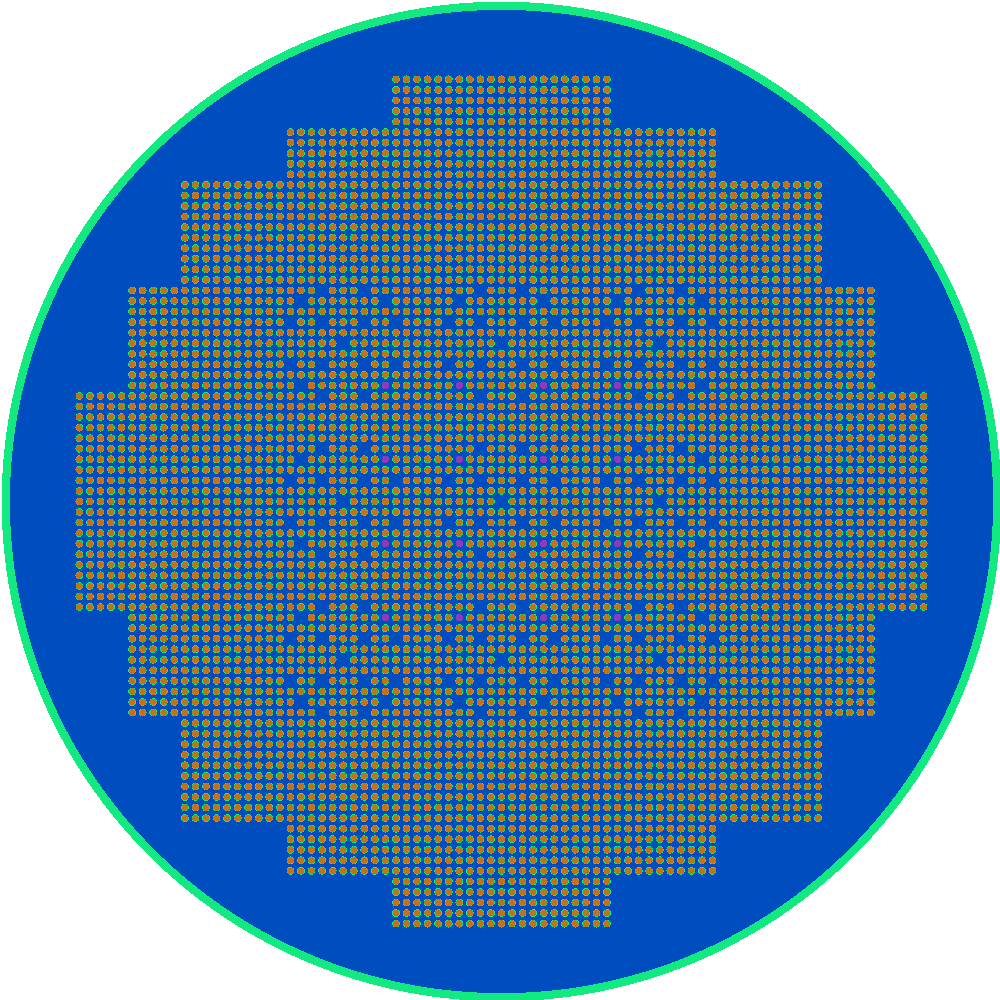
\includegraphics[width=2in]{src/plots/1_material_coloring.png}
      \column{3.5in}
      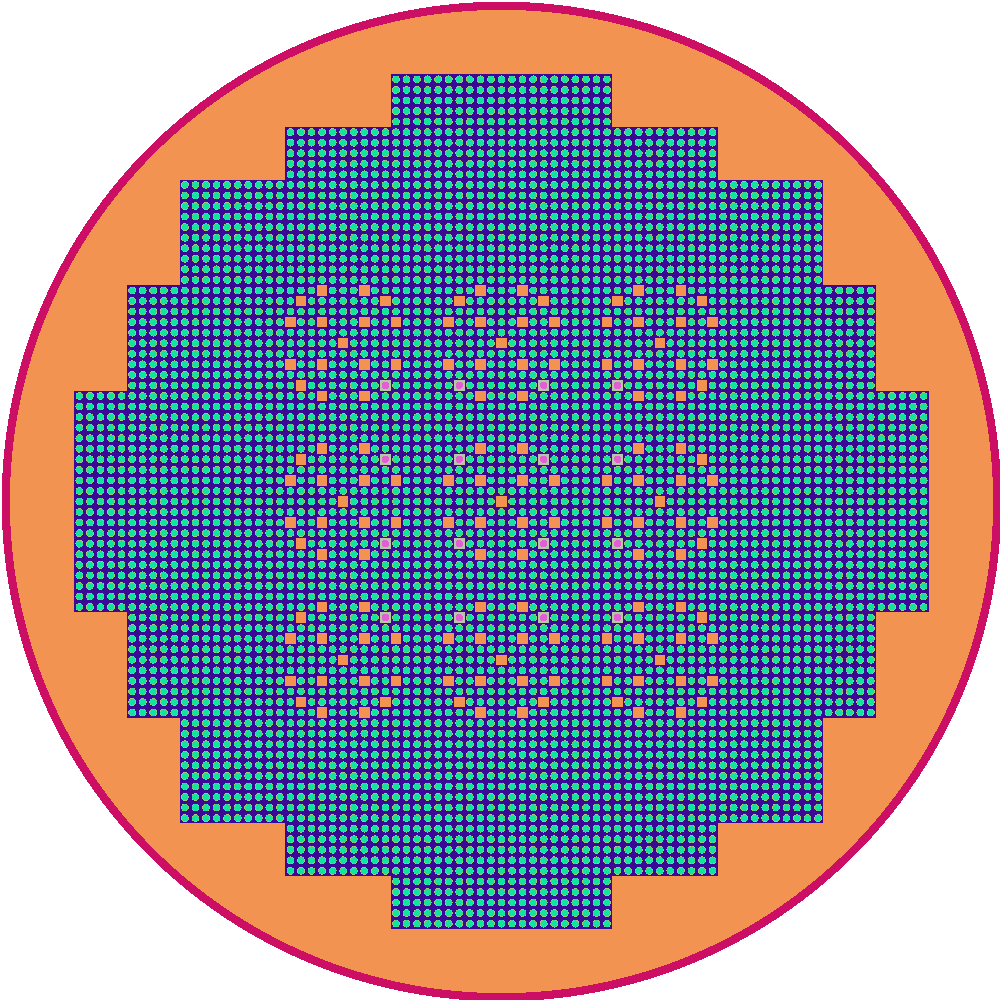
\includegraphics[width=2in]{src/plots/2_cell_coloring.png}
      \end{columns}
    \end{textblock}
  }
  
\end{frame}

%-------------------------------------------------------------------------------

\begin{frame}[fragile]{Plotting Options}

  \begin{scriptsize}
    \begin{lstlisting}[language=XML,gobble=4]
      <?xml version="1.0"?>
      <plots>

      <plot id="4" type="slice" color="mat">
        <filename>col_spec</filename>
        <origin>0 0 0</origin>
        <width>155 155</width>
        <basis>xy</basis>
        <pixels>2000 2000</pixels>
        <!-- Change background color to black -->
        <!-- This is the color used where no cell is found -->
        <background>0 0 0</background>
        <!-- Specify material colors -->
        <col_spec id="1" rgb="0 0 255"/>      <!-- Water: blue -->
        <col_spec id="2" rgb="255 0 0"/>      <!-- Fuel:  red  -->
        <col_spec id="3" rgb="160 160 160"/>  <!-- Clad:  gray -->
        <!--The remaining material colors will be randomly selected -->
      </plot>

      </plots>
    \end{lstlisting}
  \end{scriptsize}

  \begin{itemize}
    \item Can specify colors for cells or materials manually
  \end{itemize}
  
  \onslide<2>{
    \setlength{\TPHorizModule}{\framewidth}
    \setlength{\TPVertModule}{\paperheight}
    \begin{textblock}{1}(0.12,-0.645)
      \begin{columns}[c]
      \column{2in}
      \column{3.5in}
      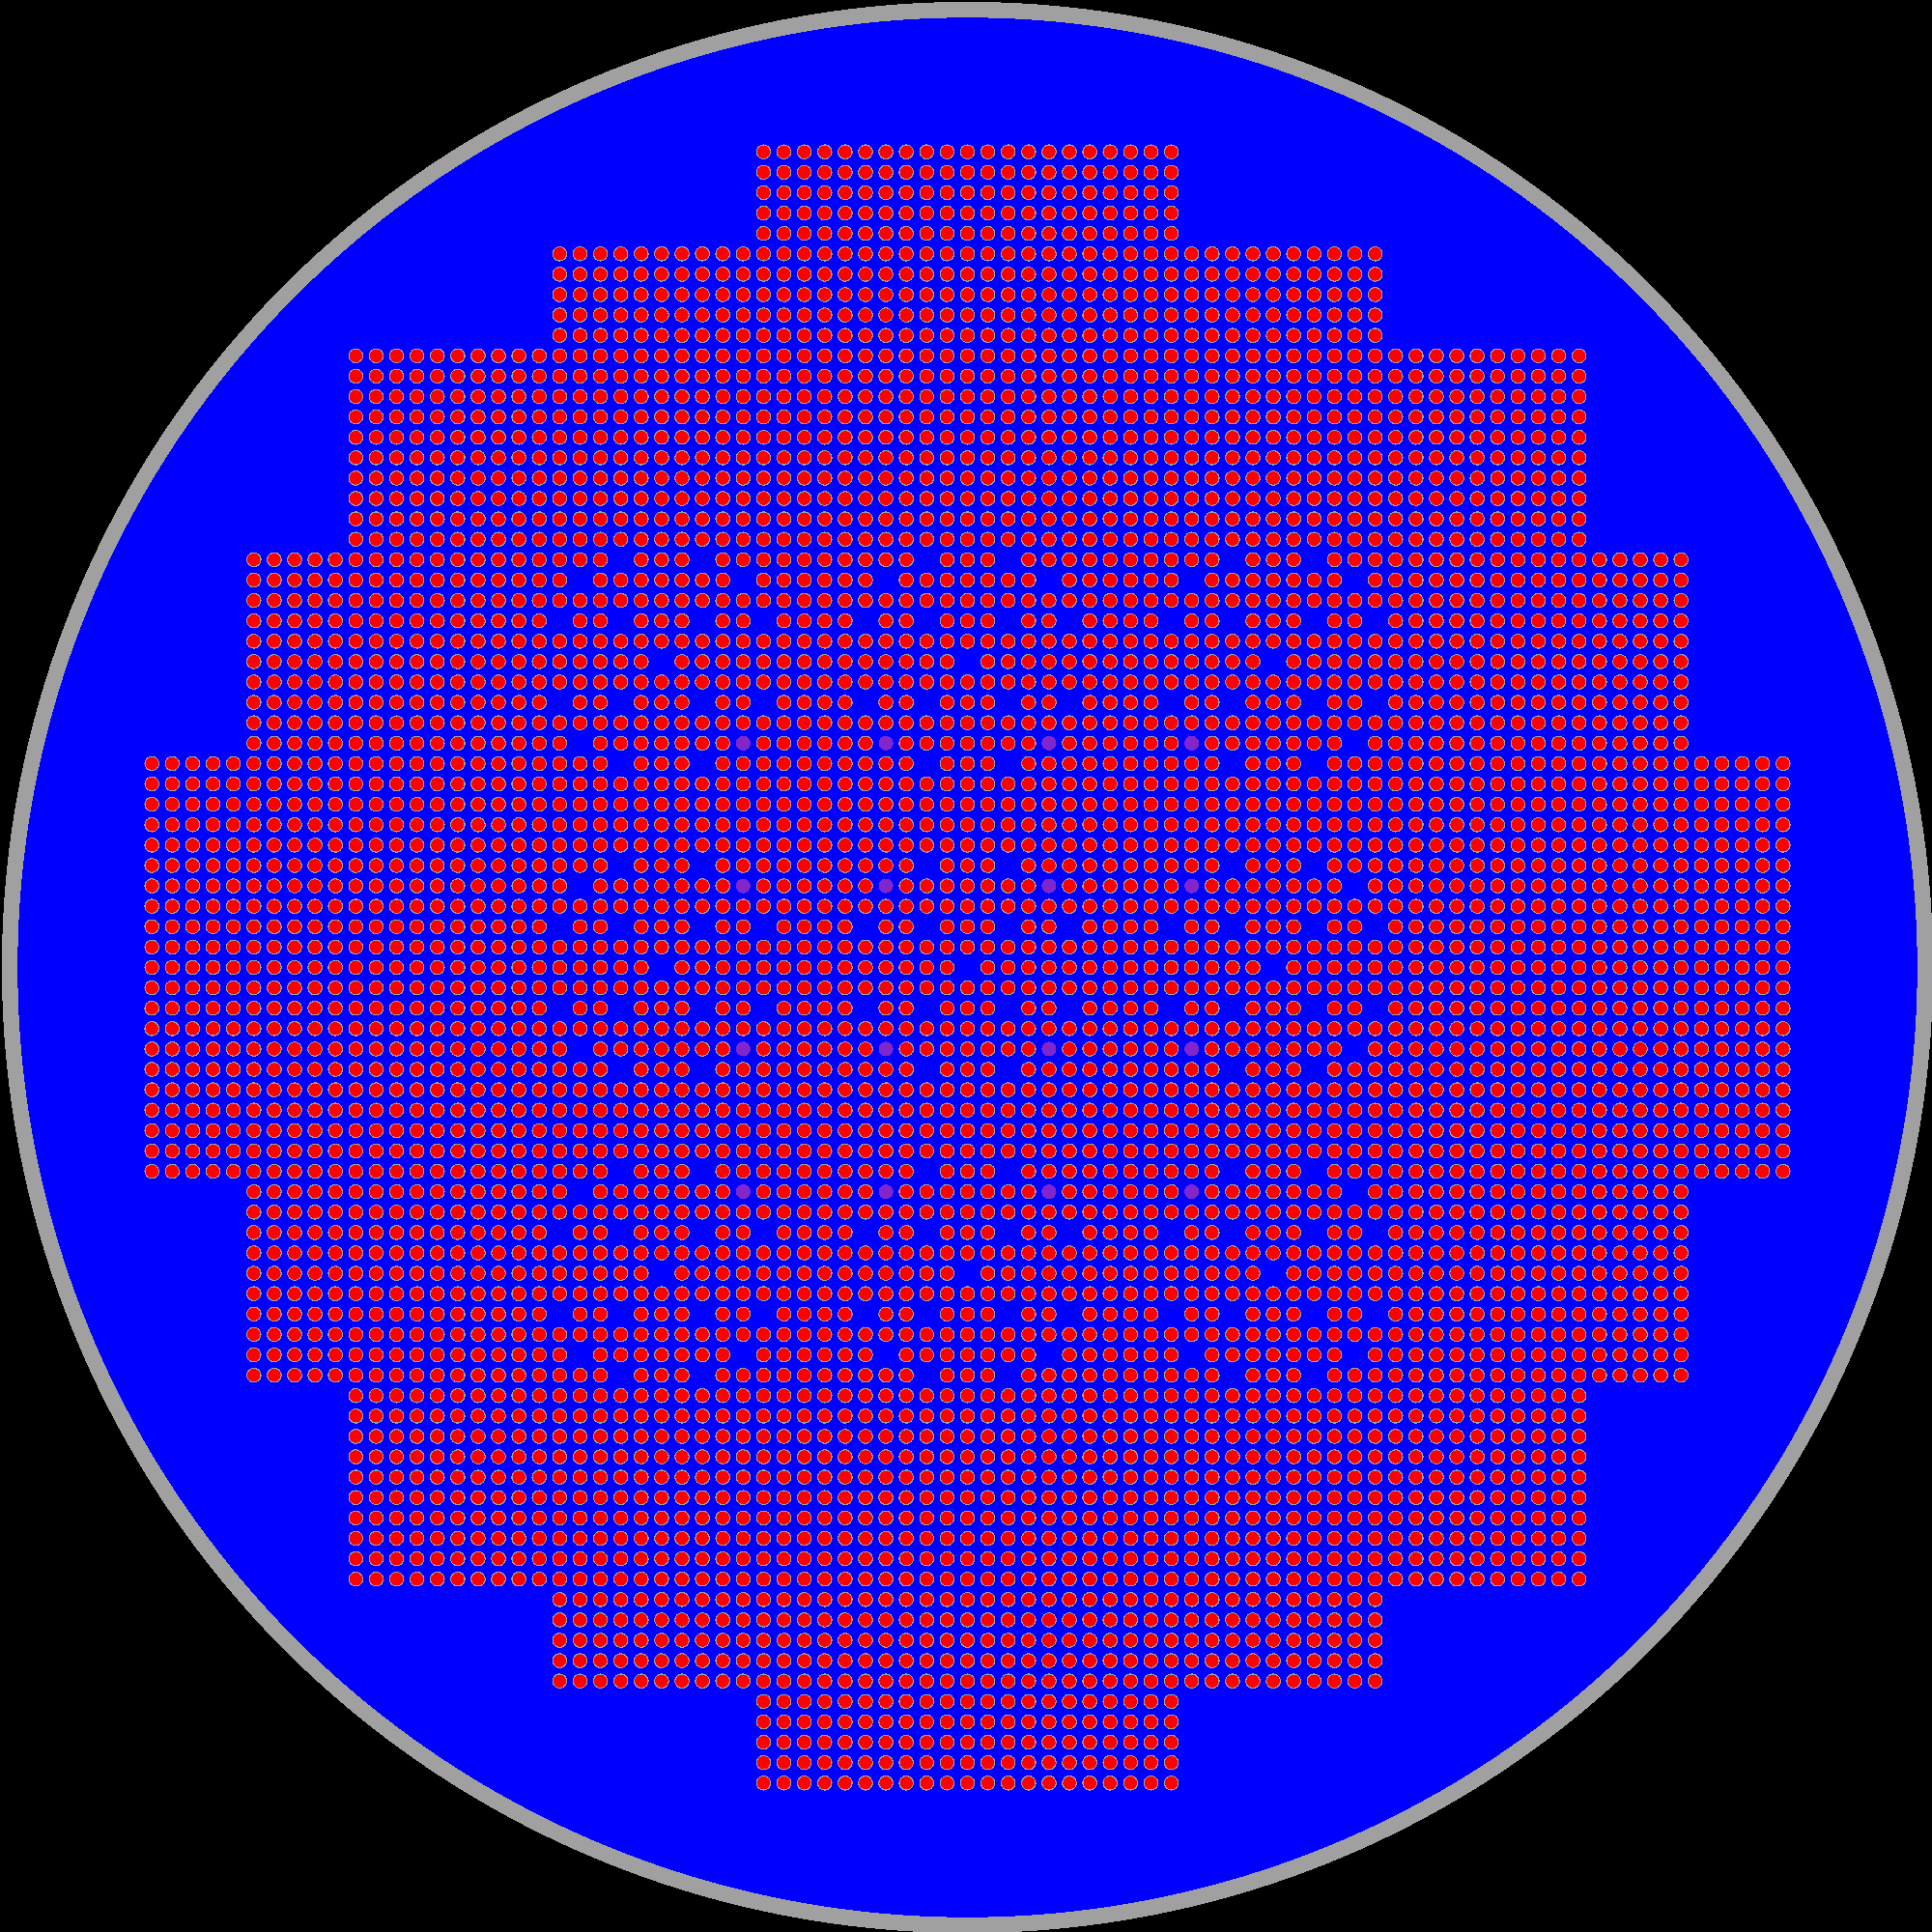
\includegraphics[width=2in]{src/plots/4_col_spec.png}
      \end{columns}
    \end{textblock}
  }
  
\end{frame}

%-------------------------------------------------------------------------------

\begin{frame}[fragile]{Plotting Options}

  \begin{scriptsize}
    \begin{lstlisting}[language=XML,gobble=4]
      <?xml version="1.0"?>
      <plots>
      
        <!-- Use a mask to plot only specific cells -->
        <plot id="5" type="slice" color="cell">
          <filename>col_spec</filename>
          <origin>0 0 0</origin>
          <width>155 155</width>
          <basis>xy</basis>
          <pixels>2000 2000</pixels>
          
          <!-- Here we plot only cells 31 and 1112, coloring all other cells white -->
          <mask components="31 1112" background="255 255 255"/>
          
          <!-- We can still set specific colors while using a mask -->
          <col_spec id="31" rgb="0 255 0"/>      <!-- Control: green  -->
          <col_spec id="1112" rgb="0 0 0"/>      <!-- Barrel:  black  -->
          
          <!-- we can still set the background color when using a mash -->
          <background>0 255 255</background>
        </plot>

      </plots>
    \end{lstlisting}
  \end{scriptsize}

  \begin{itemize}
    \item Use a mask to isolate features of interest
  \end{itemize}
  
  \onslide<2>{
    \setlength{\TPHorizModule}{\framewidth}
    \setlength{\TPVertModule}{\paperheight}
    \begin{textblock}{1}(0.12,-0.68)
      \begin{columns}[c]
      \column{2in}
      \column{3.5in}
      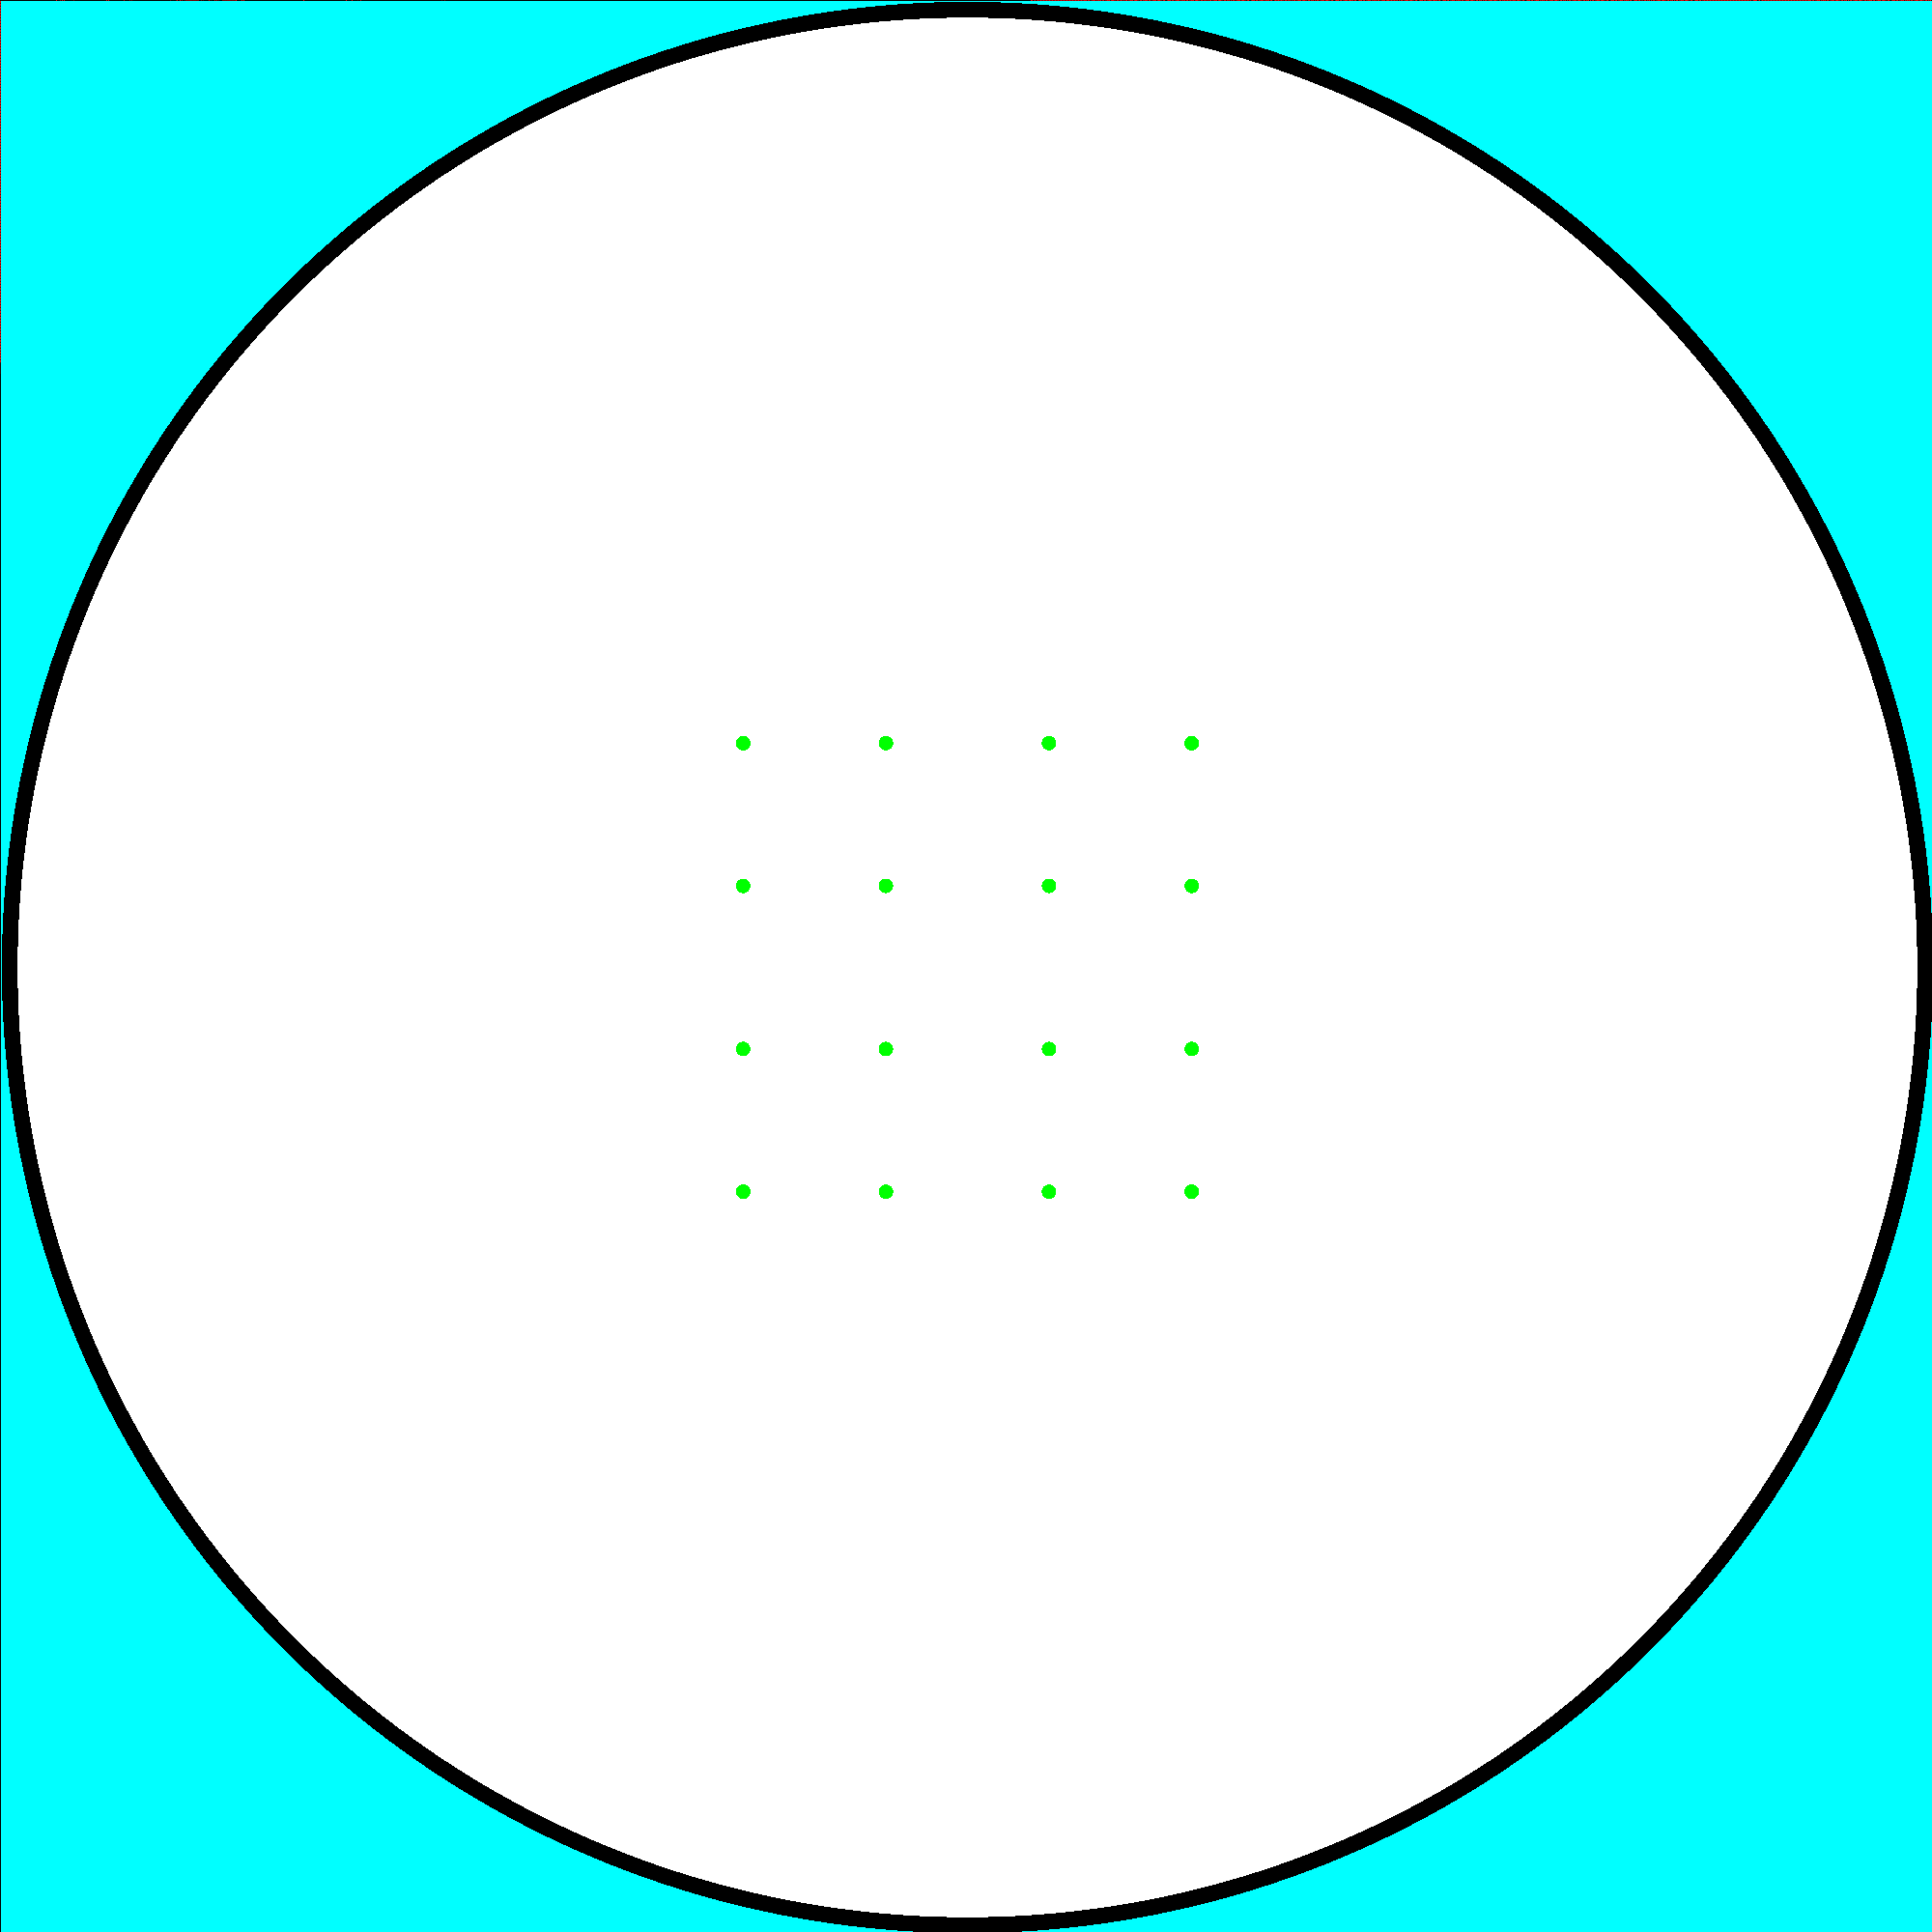
\includegraphics[width=2in]{src/plots/5_col_spec.png}
      \end{columns}
    \end{textblock}
  }
  
\end{frame}


%-------------------------------------------------------------------------------

\begin{frame}{Questions?}

      \centering
      
      Now you can model anything with OpenMC!
      
      \vspace{0.3cm}
      
      User's Guide: http://mit-crpg.github.com/openmc/
      
      \vspace{0.5cm}
      
      \begin{columns}
        \begin{column}{0.5\linewidth}
          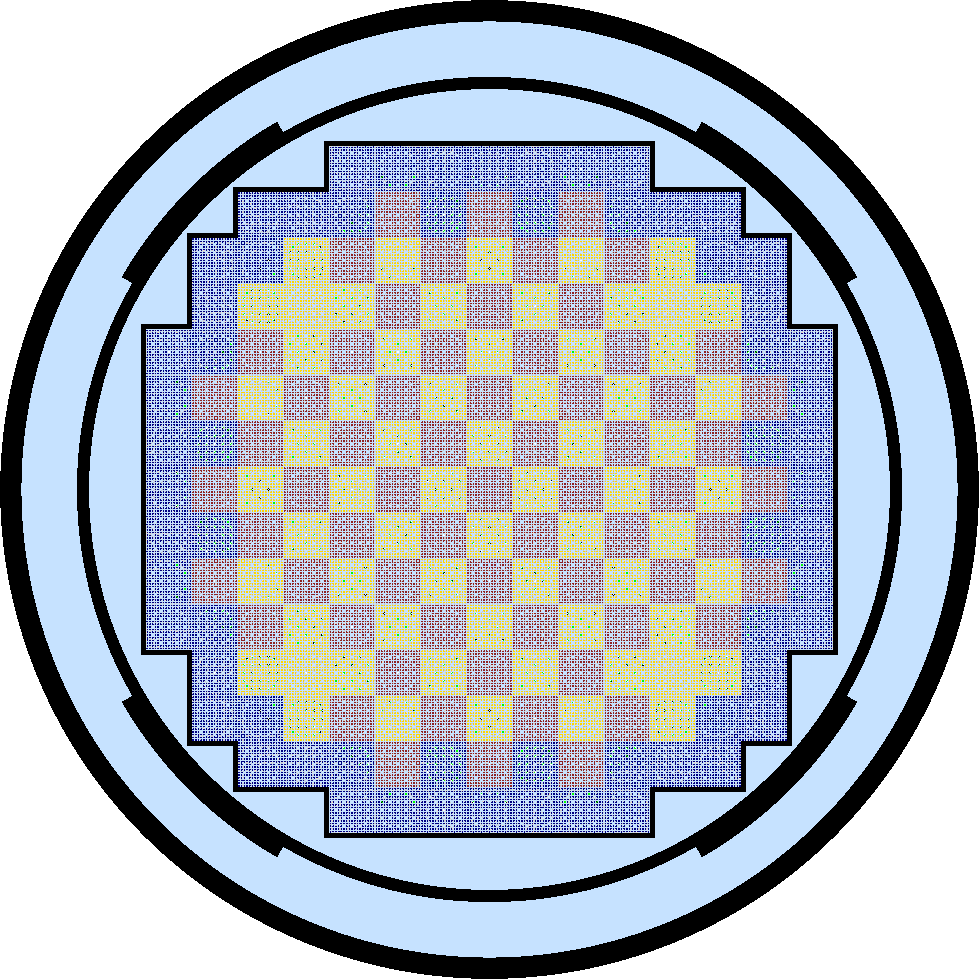
\includegraphics[width=2in]{src/core.png}
        \end{column}
        \begin{column}{0.5\linewidth}
          \centering
          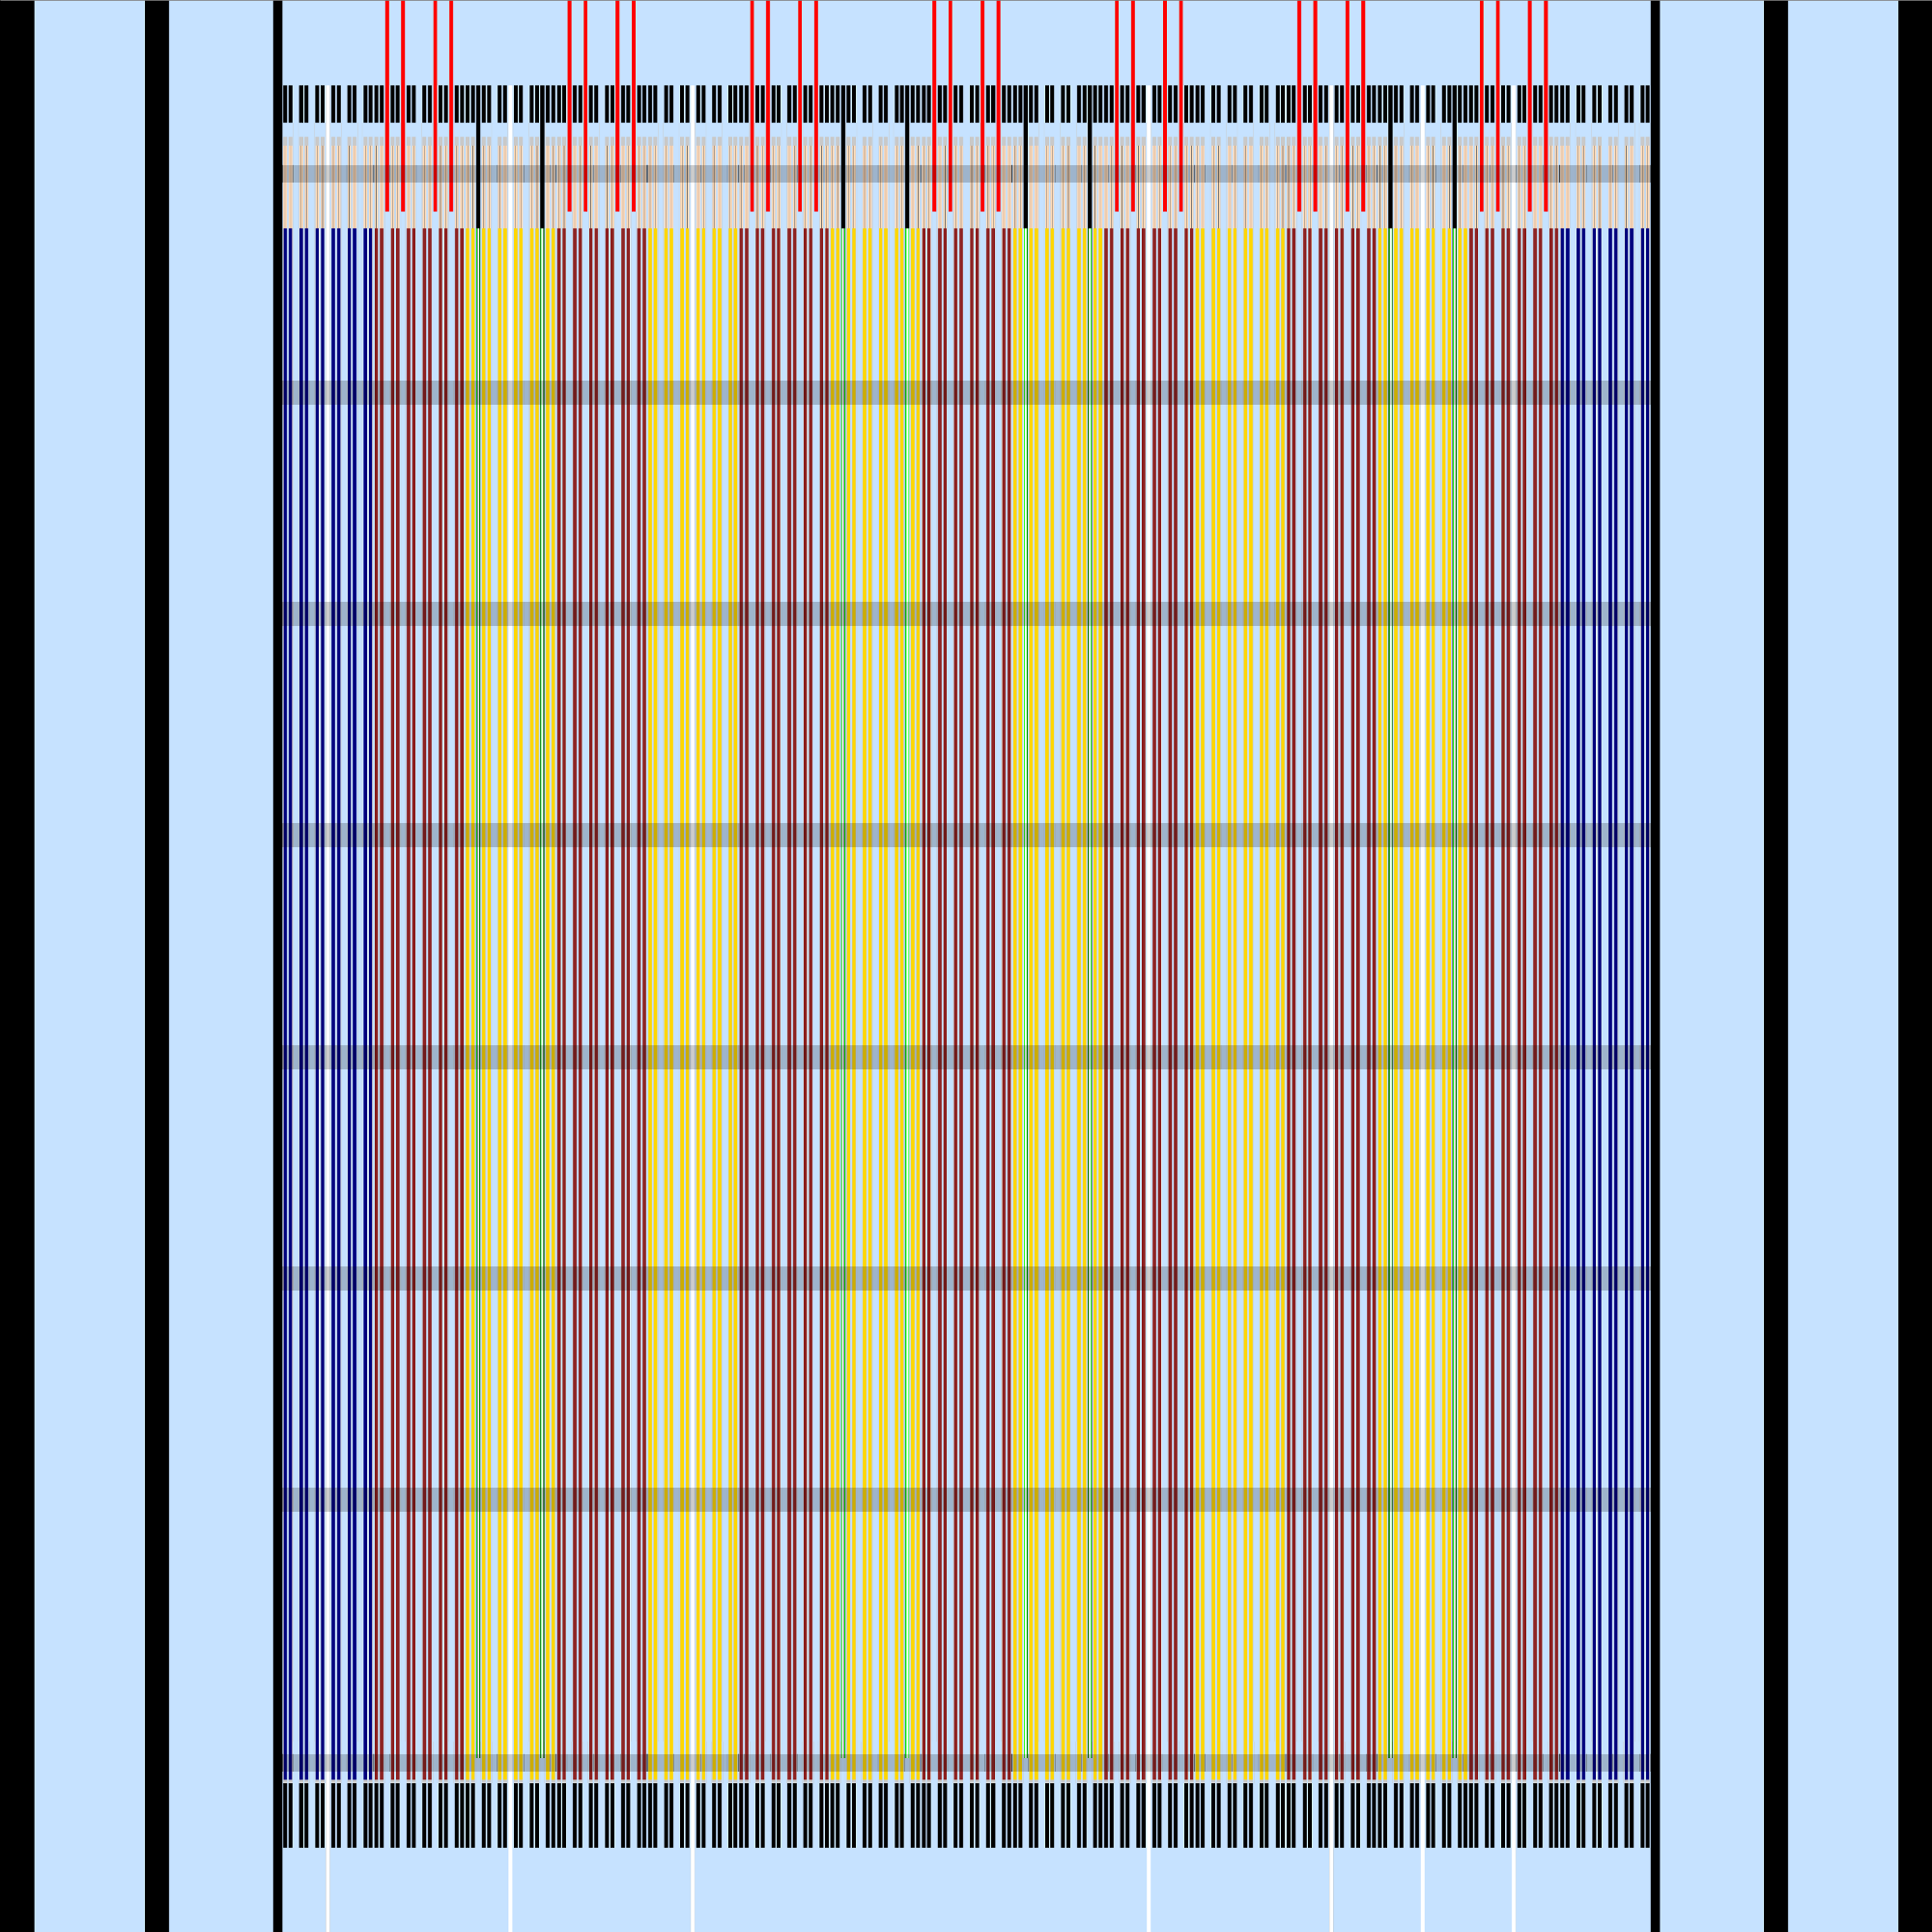
\includegraphics[width=2in]{src/axial.png}      
        \end{column}
      \end{columns}
      
\end{frame}

%-------------------------------------------------------------------------------
\end{document}
%-------------------------------------------------------------------------------
